\subsection{Themis: I/O-Efficient MapReduce}
\label{sec:themis}

In this section, we present a brief overview of \themis, our highly
I/O-efficient MapReduce system. A more detailed description and evaluation of
\themis is presented in ~\cite{themis}.  We opted to implement our fault
tolerance scheme in \themis rather than Hadoop because \themis lacked a
proportional fault tolerance mechanism prior to this work, whereas the
task-level fault tolerance scheme used by Hadoop is a tightly-integrated part
of its design.

 \themis is designed to minimize the amount of disk I/O it
 performs. Particularly, \themis tries to maintain what we call the \emph{2-IO
   property} during failure-free operation; that is, it reads and writes each
 record it processes exactly twice. In I/O-bound workloads, the performance of
 a system is limited by the speed at which it can write to secondary storage
 and the number of times it writes to that storage. Aggarwal and
 Vitter~\cite{sort-io} show that two reads and two writes per record is a lower
 bound for large-scale distributed sorting, and since a distributed sort by key
 forms the kernel of MapReduce computations, this bound applies to MapReduce as
 well. Hence, by achieving the 2-IO property, \themis minimizes the amount of
 disk I/O it performs.

\begin{figure}
  \centering
  \begin{subfigure}[t]{\columnwidth}
  \centering
  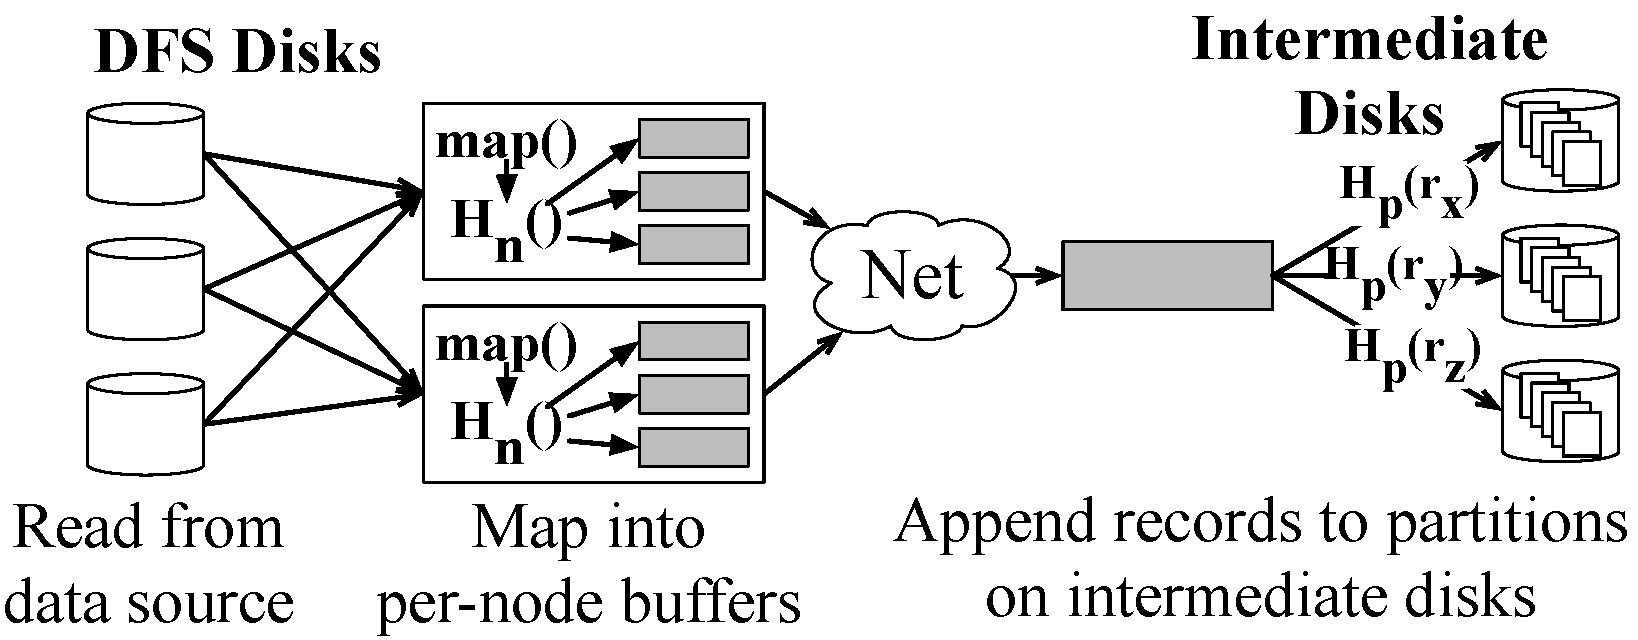
\includegraphics[width=\columnwidth]{fault_tolerance/figures/detailed_phase_one.pdf}
  \caption{\label{fig:phase_one} Phase One}
  \end{subfigure}\vspace{1em}
  \begin{subfigure}[t]{\columnwidth}
  \centering
  
\includegraphics[width=\columnwidth]{fault_tolerance/figures/phase_two.pdf}
  \caption{\label{fig:phase_two} Phase Two}
  \end{subfigure}

  \caption{\label{fig:themis_phases} A diagrammatic overview of \themis' phases.}
\end{figure}

Nodes in a \themis cluster each have a collection of \emph{intermediate disks}
that store volatile intermediate data and a disjoint collection of \emph{DFS
  disks} that store input and output data, and are typically under the control
of a distributed file system like HDFS.

\themis runs a MapReduce job in two main \emph{phases}, called \emph{phase one}
and \emph{phase two}.  In phase one, input records are read in parallel from
the cluster's DFS disks. \themis applies the \map function to each record,
producing a collection of \emph{intermediate records} that are written to
intermediate partitions spread across the cluster's intermediate disks. Each
intermediate partition holds all records with a certain set of keys. The
mapping from keys to intermediate partitions is determined by a \emph{partition
  function}. Phase one is roughly analogous to Hadoop's map and shuffle phases.

At the end of phase one, all intermediate records have been generated,
partitioned and stored across the cluster's intermediate disks. A diagrammatic
overview of phase one is given in Figure~\ref{fig:phase_one}.

In phase two, each intermediate partition is read from the cluster's
intermediate disks completely into memory. Once in memory, it is sorted in-core
by key, and the \reduce function is applied to each group of records in the
partition with the same key. This produces a collection of \emph{output
  records} that are written to files on the DFS disks. Phase two is roughly
equivalent to Hadoop's sort and reduce phases. A diagrammatic overview of phase
two is given in Figure~\ref{fig:phase_two}.

Note that phase one requires all-to-all communication among cluster nodes, but
that phase two can be executed on each node independently.

\subsubsection{Partitioning}

In order for phase two to be processed efficiently, partitions should be small
enough for several of them to be processed in memory
simultaneously. Additionally, they should be as uniformly-sized as possible to
prevent stragglers. The partition function is responsible for ensuring both
these properties. The user can provide their own partition function, or it can
be derived at runtime through an optional sampling phase called \emph{phase
  zero}. Phase zero requires a fairly small sample to produce a good partition
function, and typically takes under a minute to run.
